\documentclass{standalone}
\usepackage{tikz}
\usetikzlibrary{patterns}
\usetikzlibrary{positioning}
\usetikzlibrary{patterns, positioning}
\usetikzlibrary{shapes.misc}
\usepackage[outline]{contour}
\contourlength{1.5pt} 
\usepackage[sfdefault]{ClearSans}

\begin{document}
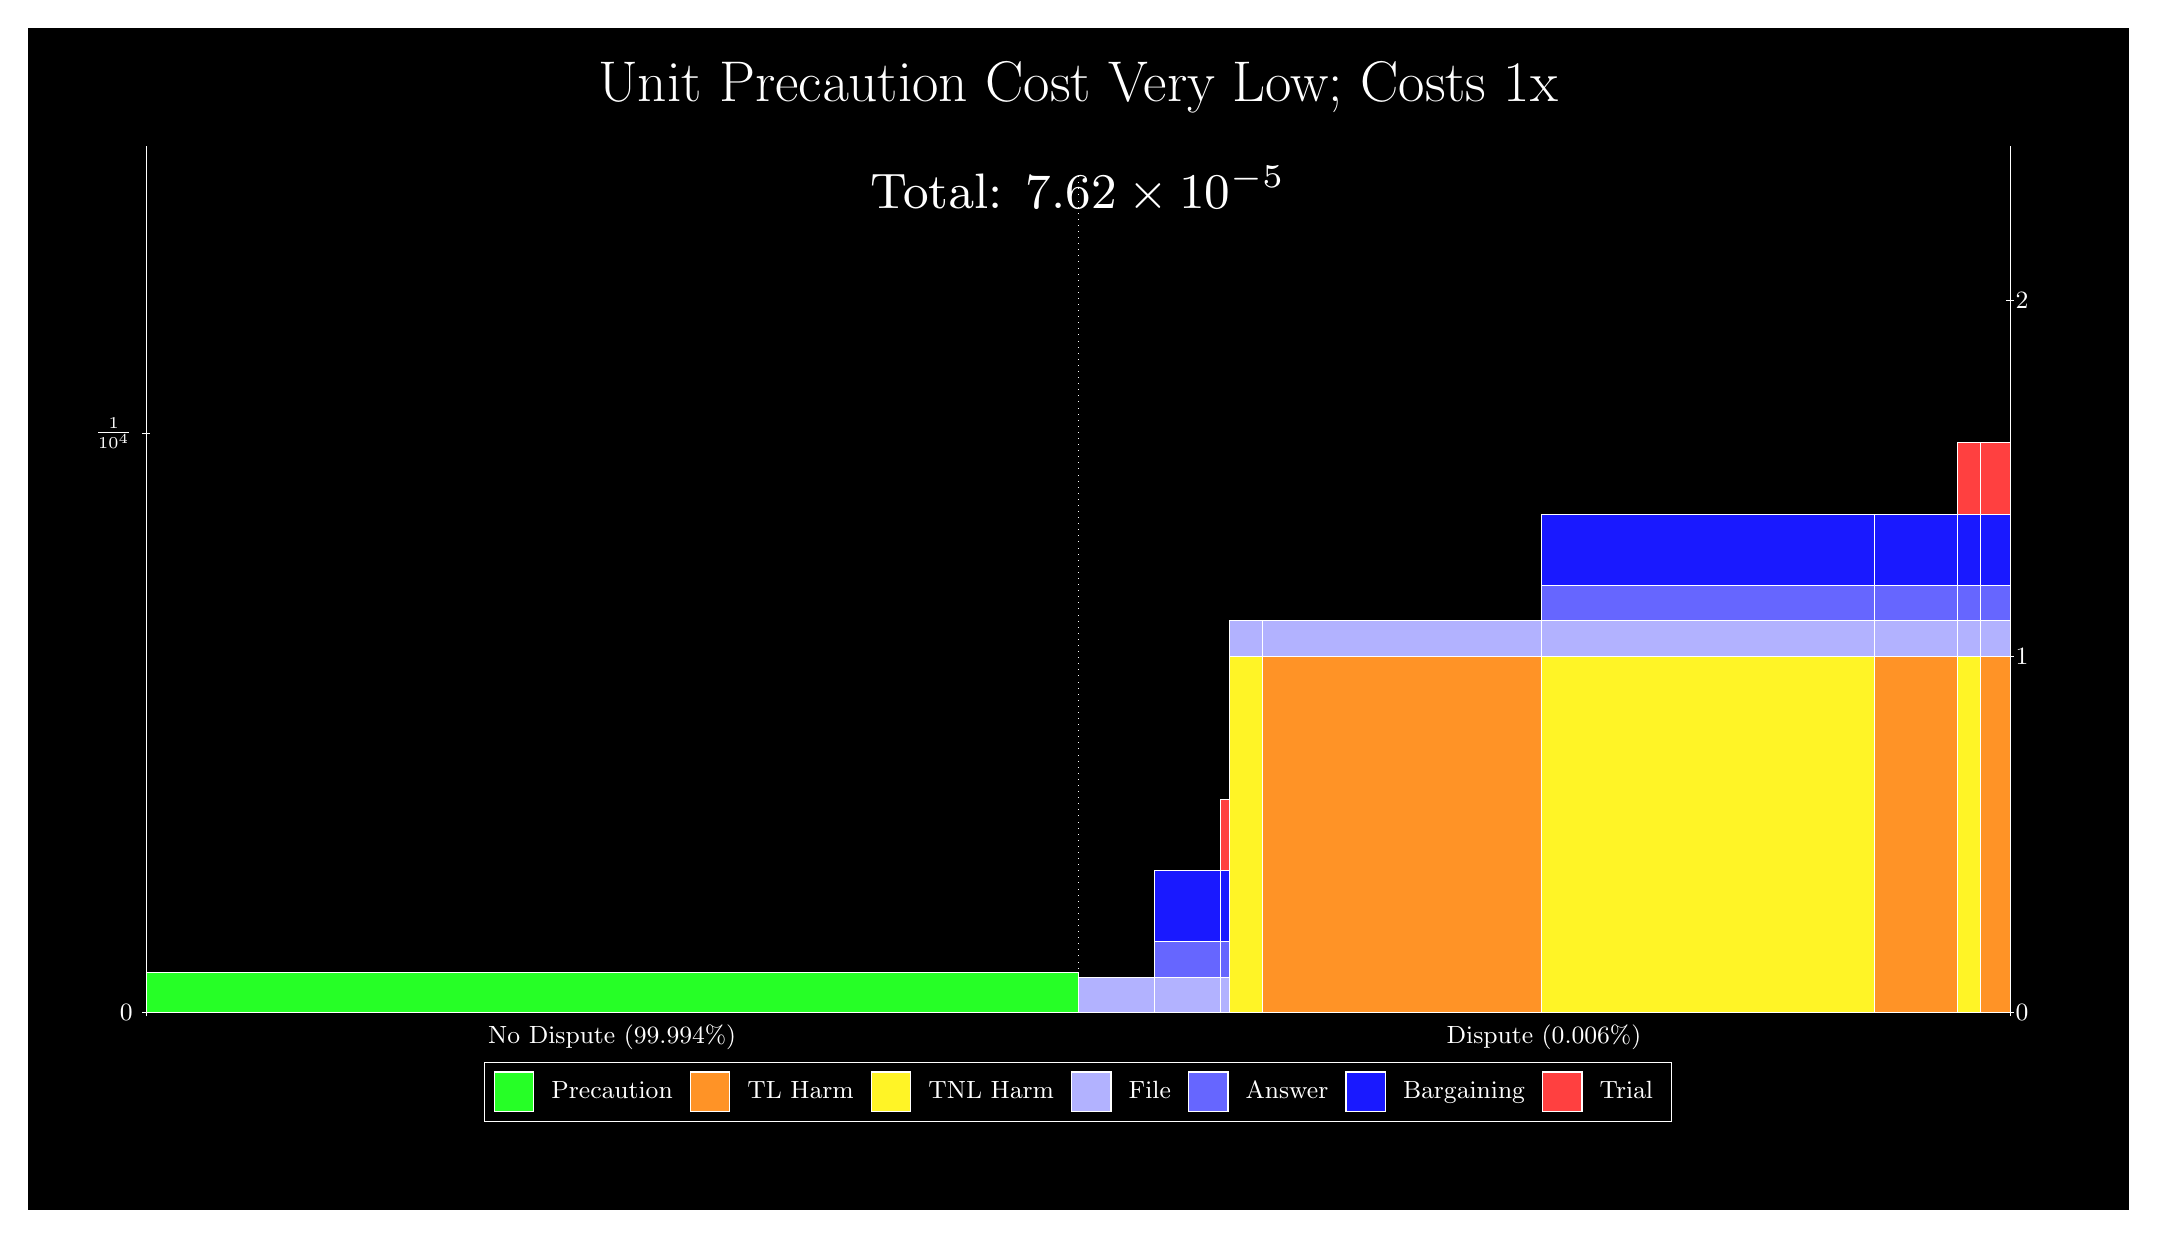
\begin{tikzpicture}
\draw[fill=black] (0,0) rectangle (26.667,15);
\draw[draw=none,text=white] (0,13.5) rectangle (26.667,15) node[midway] {\huge Unit Precaution Cost Very Low; Costs 1x};
\draw[fill=green!85,draw=white,very thin] (1.5,2.5) rectangle (13.333,3.015);
\draw[fill=green!85,draw=white,very thin] (13.333,2.5) rectangle (14.303,2.5);
\draw[fill=blue!30,draw=white,very thin] (13.333,2.5) rectangle (14.303,2.9523);
\draw[fill=green!85,draw=white,very thin] (14.303,2.5) rectangle (15.138,2.5);
\draw[fill=blue!30,draw=white,very thin] (14.303,2.5) rectangle (15.138,2.9523);
\draw[fill=blue!60,draw=white,very thin] (14.303,2.9523) rectangle (15.138,3.4046);
\draw[fill=blue!90,draw=white,very thin] (14.303,3.4046) rectangle (15.138,4.3091);
\draw[fill=green!85,draw=white,very thin] (15.138,2.5) rectangle (15.259,2.5);
\draw[fill=blue!30,draw=white,very thin] (15.138,2.5) rectangle (15.259,2.9523);
\draw[fill=blue!60,draw=white,very thin] (15.138,2.9523) rectangle (15.259,3.4046);
\draw[fill=blue!90,draw=white,very thin] (15.138,3.4046) rectangle (15.259,4.3091);
\draw[fill=red!75,draw=white,very thin] (15.138,4.3091) rectangle (15.259,5.2137);
\draw[fill=green!85,draw=white,very thin] (15.259,2.5) rectangle (15.672,2.5);
\draw[fill=yellow!85,draw=white,very thin] (15.259,2.5) rectangle (15.672,7.0227);
\draw[fill=blue!30,draw=white,very thin] (15.259,7.0227) rectangle (15.672,7.475);
\draw[fill=green!85,draw=white,very thin] (15.672,2.5) rectangle (19.21,2.5);
\draw[fill=orange!85,draw=white,very thin] (15.672,2.5) rectangle (19.21,7.0227);
\draw[fill=blue!30,draw=white,very thin] (15.672,7.0227) rectangle (19.21,7.475);
\draw[fill=green!85,draw=white,very thin] (19.21,2.5) rectangle (23.444,2.5);
\draw[fill=yellow!85,draw=white,very thin] (19.21,2.5) rectangle (23.444,7.0227);
\draw[fill=blue!30,draw=white,very thin] (19.21,7.0227) rectangle (23.444,7.475);
\draw[fill=blue!60,draw=white,very thin] (19.21,7.475) rectangle (23.444,7.9273);
\draw[fill=blue!90,draw=white,very thin] (19.21,7.9273) rectangle (23.444,8.8318);
\draw[fill=green!85,draw=white,very thin] (23.444,2.5) rectangle (24.497,2.5);
\draw[fill=orange!85,draw=white,very thin] (23.444,2.5) rectangle (24.497,7.0227);
\draw[fill=blue!30,draw=white,very thin] (23.444,7.0227) rectangle (24.497,7.475);
\draw[fill=blue!60,draw=white,very thin] (23.444,7.475) rectangle (24.497,7.9273);
\draw[fill=blue!90,draw=white,very thin] (23.444,7.9273) rectangle (24.497,8.8318);
\draw[fill=green!85,draw=white,very thin] (24.497,2.5) rectangle (24.794,2.5);
\draw[fill=yellow!85,draw=white,very thin] (24.497,2.5) rectangle (24.794,7.0227);
\draw[fill=blue!30,draw=white,very thin] (24.497,7.0227) rectangle (24.794,7.475);
\draw[fill=blue!60,draw=white,very thin] (24.497,7.475) rectangle (24.794,7.9273);
\draw[fill=blue!90,draw=white,very thin] (24.497,7.9273) rectangle (24.794,8.8318);
\draw[fill=red!75,draw=white,very thin] (24.497,8.8318) rectangle (24.794,9.7364);
\draw[fill=green!85,draw=white,very thin] (24.794,2.5) rectangle (25.167,2.5);
\draw[fill=orange!85,draw=white,very thin] (24.794,2.5) rectangle (25.167,7.0227);
\draw[fill=blue!30,draw=white,very thin] (24.794,7.0227) rectangle (25.167,7.475);
\draw[fill=blue!60,draw=white,very thin] (24.794,7.475) rectangle (25.167,7.9273);
\draw[fill=blue!90,draw=white,very thin] (24.794,7.9273) rectangle (25.167,8.8318);
\draw[fill=red!75,draw=white,very thin] (24.794,8.8318) rectangle (25.167,9.7364);
\node[font=\small,text=white,anchor=north,scale=2] at (13.333, 13.5) {Total: $7.62\times 10^{-5}$};
\draw[white,very thin] (1.5,2.5) -- (1.5,13.5);
\draw[white,very thin] (1.45,2.5) -- (1.55,2.5);
\node[font=\small,text=white, anchor=east] at (1.45, 2.5) {0};
\draw[white,very thin] (1.45,9.8575) -- (1.55,9.8575);
\node[font=\small,text=white, anchor=east] at (1.45, 9.8575) {$\frac{1}{10^{4}}$};

\draw[white,dotted,very thin] (13.333,2.83) -- (13.333,13.17);
\draw[white,very thin] (25.167,2.5) -- (25.167,13.5);
\draw[white,very thin] (25.117,2.5) -- (25.217,2.5);
\node[font=\small,text=white, anchor=west] at (25.117, 2.5) {0};
\draw[white,very thin] (25.117,7.0227) -- (25.217,7.0227);
\node[font=\small,text=white, anchor=west] at (25.117, 7.0227) {1};
\draw[white,very thin] (25.117,11.545) -- (25.217,11.545);
\node[font=\small,text=white, anchor=west] at (25.117, 11.545) {2};

\draw[white,very thin] (1.5,2.5) -- (25.167,2.5);
\draw[white,very thin] (1.5,2.45) -- (1.5,2.55);
\node[font=\small,text=white, anchor=north] at (1.5, 2.45) {};
\draw[white,very thin] (25.167,2.45) -- (25.167,2.55);
\node[font=\small,text=white, anchor=north] at (25.167, 2.45) {};

\node[font=\small,text=white,anchor=south] at (7.4167, 1.9) {No\ Dispute\ (99.994\%)};
\node[font=\small,text=white,anchor=south] at (19.25, 1.9) {Dispute\ (0.006\%)};
\draw (13.3333,2.5) node (B) {};
\begin{scope}[align=center]
\matrix[scale=0.5,draw=white,below=0.5cm of B,nodes={draw},column sep=0.1cm]{
\node[rectangle,draw,minimum width=0.5cm,minimum height=0.5cm,fill=green!85]{}; & \node[draw=none,font=\small,text=white]{Precaution}; &
\node[rectangle,draw,minimum width=0.5cm,minimum height=0.5cm,fill=orange!85]{}; & \node[draw=none,font=\small,text=white]{TL Harm}; &
\node[rectangle,draw,minimum width=0.5cm,minimum height=0.5cm,fill=yellow!85]{}; & \node[draw=none,font=\small,text=white]{TNL Harm}; &
\node[rectangle,draw,minimum width=0.5cm,minimum height=0.5cm,fill=blue!30]{}; & \node[draw=none,font=\small,text=white]{File}; &
\node[rectangle,draw,minimum width=0.5cm,minimum height=0.5cm,fill=blue!60]{}; & \node[draw=none,font=\small,text=white]{Answer}; &
\node[rectangle,draw,minimum width=0.5cm,minimum height=0.5cm,fill=blue!90]{}; & \node[draw=none,font=\small,text=white]{Bargaining}; &
\node[rectangle,draw,minimum width=0.5cm,minimum height=0.5cm,fill=red!75]{}; & \node[draw=none,font=\small,text=white]{Trial}; \\\\
};\end{scope}

\end{tikzpicture}
\end{document}